\section{User Managament elements}

Some elements have been created for user managment.
Both style and behavior of these elements have been developed , so that every user can easily customize it at will and choose to use either one side or both sides of the element.
The main elements are the ones developed for the management as: login, logout, signup and reset.
The specifications for each element are indicated below.

\subsubsection{\texttt{<api-user-login>}}

Login a user with the given credentials.
\begin{lstlisting}[language=html]
<api-user-login credentials="{{credentials}}"
collection="{{collection}}" 
response="{{response}}" error="{{error}}"/>
\end{lstlisting}
Where:
\begin{itemize}
\item \texttt{credentials} email and password of user.
\item \texttt{collection} name of collection(Object).
\item \texttt{response}	HTTP response message(String).
\item \texttt{error} object of the error response(Object).
\end{itemize}

\begin {figure}[h]
\graphicspath{{images/chapter_USR/}}
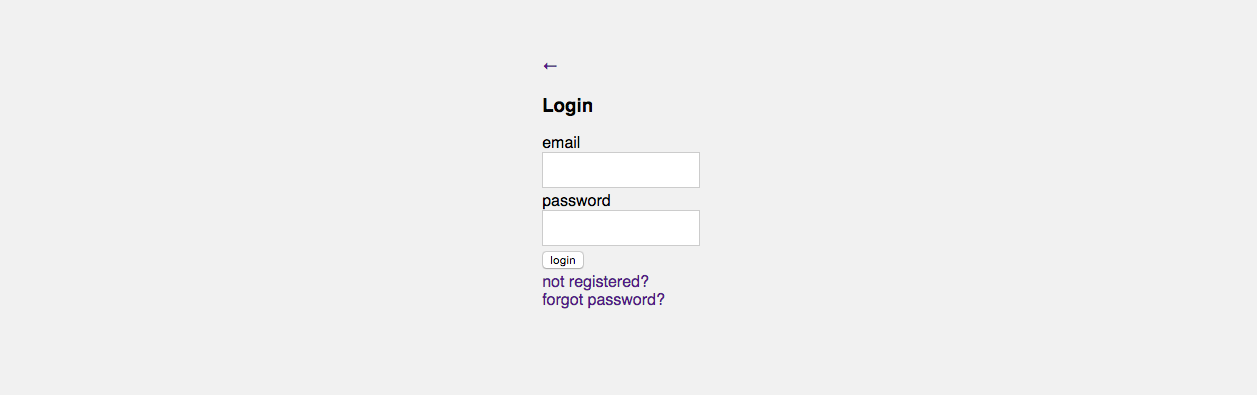
\includegraphics[width=\textwidth]{usr1}
\caption{Login Element}
\end {figure}

\subsubsection{\texttt{<api-user-logout>}}

Logout a user with the given accessToken id.
\begin{lstlisting}[language=html]
<api-user-logout collection="{{collection}}" 
response="{{response}}" error="{{error}}"/>
\end{lstlisting}
Where:
\begin{itemize}
\item \texttt{credentials} email and password of user.
\item \texttt{collection} name of collection (Object)
\item \texttt{response}	HTTP response message (String)
\item \texttt{error} object of the error response (Object)
\end{itemize}

\subsubsection{\texttt{<api-user-signup>}}

Signup a user by with the given general information.
\begin{lstlisting}[language=html]
<api-user-signup credentials="{{credentials}}"
collection="{{collection}}" 
response="{{response}}" error="{{error}}"/>
\end{lstlisting}
Where:
\begin{itemize}
\item \texttt{credentials} email, password, name and phone-number of user.
\item \texttt{collection} name of collection (Object)
\item \texttt{response}	HTTP response message (String)
\item \texttt{error} object of the error response (Object)
\end{itemize}

\begin {figure}[h]
\graphicspath{{images/chapter_USR/}}
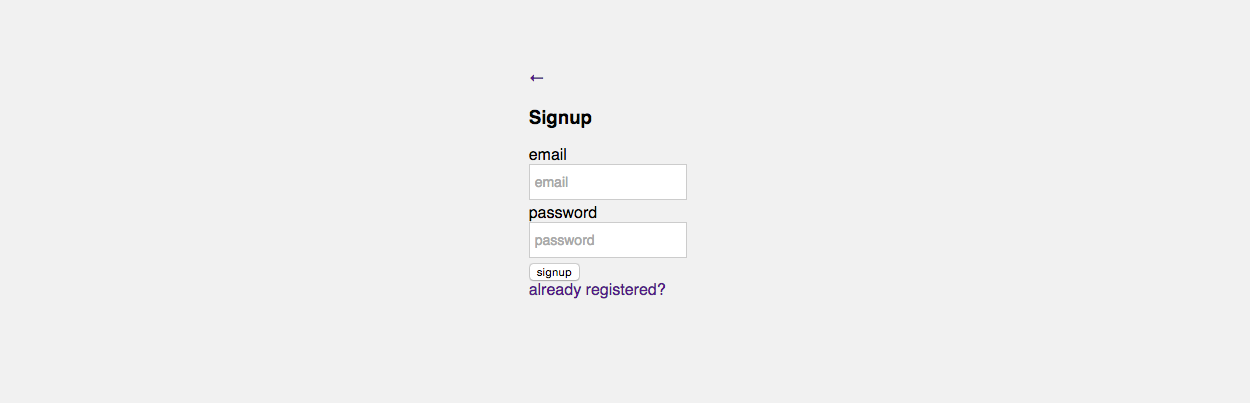
\includegraphics[width=\textwidth]{usr4}
\caption{Signup Element}
\end {figure}

\subsubsection{\texttt{<api-user-reset>}}

Create a short lived acess token for temporary login. Allows users to change passwords if forgotten.
\begin{lstlisting}[language=html]
<api-user-reset email="{{email}}"
collection="{{collection}}" 
response="{{response}}" error="{{error}}"/>
\end{lstlisting}
Where:
\begin{itemize}
\item \texttt{email} email of user (String)
\item \texttt{collection} name of collection (Object)
\item \texttt{response}	HTTP response message (String)
\item \texttt{error} object of the error response (Object)
\end{itemize}

\begin {figure}[h]
\graphicspath{{images/chapter_USR/}}
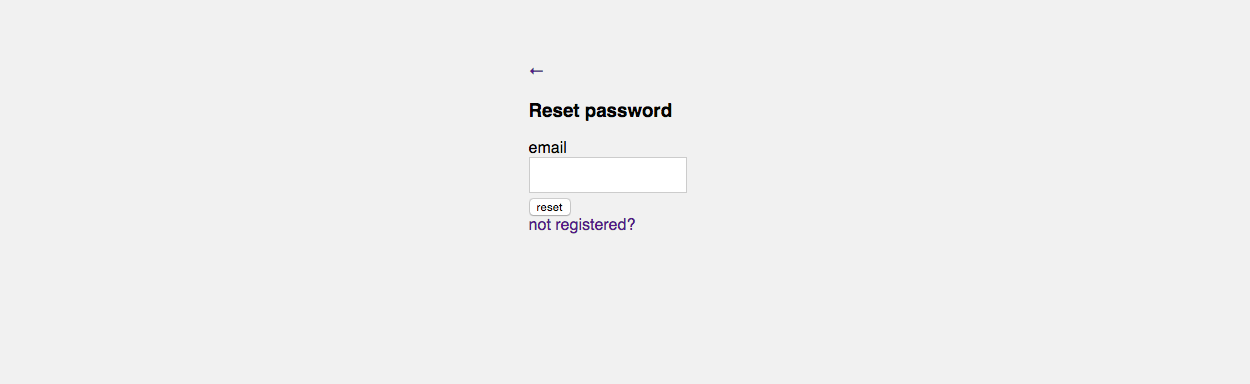
\includegraphics[width=\textwidth]{usr3}
\caption{Reset Element}
\end {figure}

\begin {figure}[h]
\graphicspath{{images/chapter_USR/}}
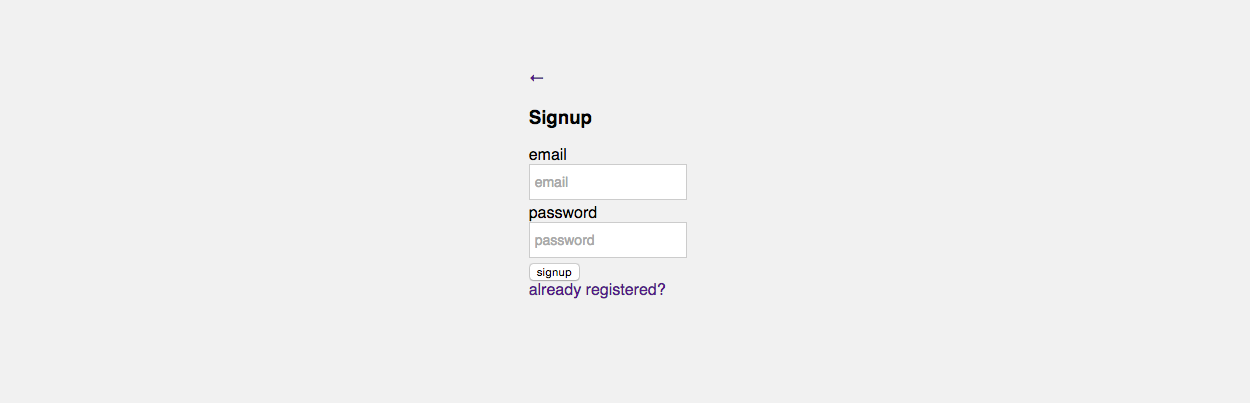
\includegraphics[width=\textwidth]{usr4}
\caption{Login Element}
\end {figure}

\subsubsection{\texttt{<form-login>}}

Create a login form.
\begin{lstlisting}[language=html]
<form id="form" on-submit="on_submit">
    <div class="field">
        <label class="label">email</label>
        <input class="input" is="iron-input" type="text" 
    		placeholder="email" 
            bind-value="{{credentials.email}}">
    </div>
    <div class="field">
        <label class="label">password</label>
        <input class="input" is="iron-input" type="password" 
        	placeholder="password" 
        	bind-value="{{credentials.password}}">
    </div>
      	<input type="submit" value="login"/>
</form>
\end{lstlisting}

\subsubsection{\texttt{<form-signup>}}

Create a signup form.
\begin{lstlisting}[language=html]
<form id="form" on-submit="on_submit">
    <div class="field">
        <label class="label">email</label>
        <input class="input" is="iron-input" type="text" 
    		placeholder="email" 
            bind-value="{{credentials.email}}">
    </div>
    <div class="field">
        <label class="label">password</label>
        <input class="input" is="iron-input" type="password" 
        	placeholder="password" 
        	bind-value="{{credentials.password}}">
    </div>
    <div class="field">
        <label class="label">firstname</label>
        <input class="input" is="iron-input" type="text" 
        	placeholder="firstname" 
        	bind-value="{{credentials.firstname}}">
    </div>
    <div class="field">
        <label class="label">lastname</label>
        <input class="input" is="iron-input" type="text" 
        	placeholder="lastname" 
        	bind-value="{{credentials.lastname}}">
    </div>
    <div class="field">
        <label class="label">phone-number</label>
        <input class="input" is="iron-input" type="text" 
        	placeholder="phone-number" 
        	bind-value="{{credentials.phone-number}}">
    </div>
      	<input type="submit" value="confirm"/>
</form>
\end{lstlisting}


\subsubsection{\texttt{<form-reset>}}

Create a reset form.
\begin{lstlisting}[language=html]
<form id="form" on-submit="on_submit">
    <div class="field">
        <label class="label">email</label>
        <input class="input" is="iron-input" type="text" 
    		placeholder="email" 
            bind-value="{{credentials.email}}">
    </div>
      	<input type="submit" value="reset"/>
</form>
\end{lstlisting}

\subsubsection{User Settings}

The User Settings is the page where it is possible to manage the personal data such as e-mail and password.

\begin {figure}[h]
\graphicspath{{images/chapter_USR/}}
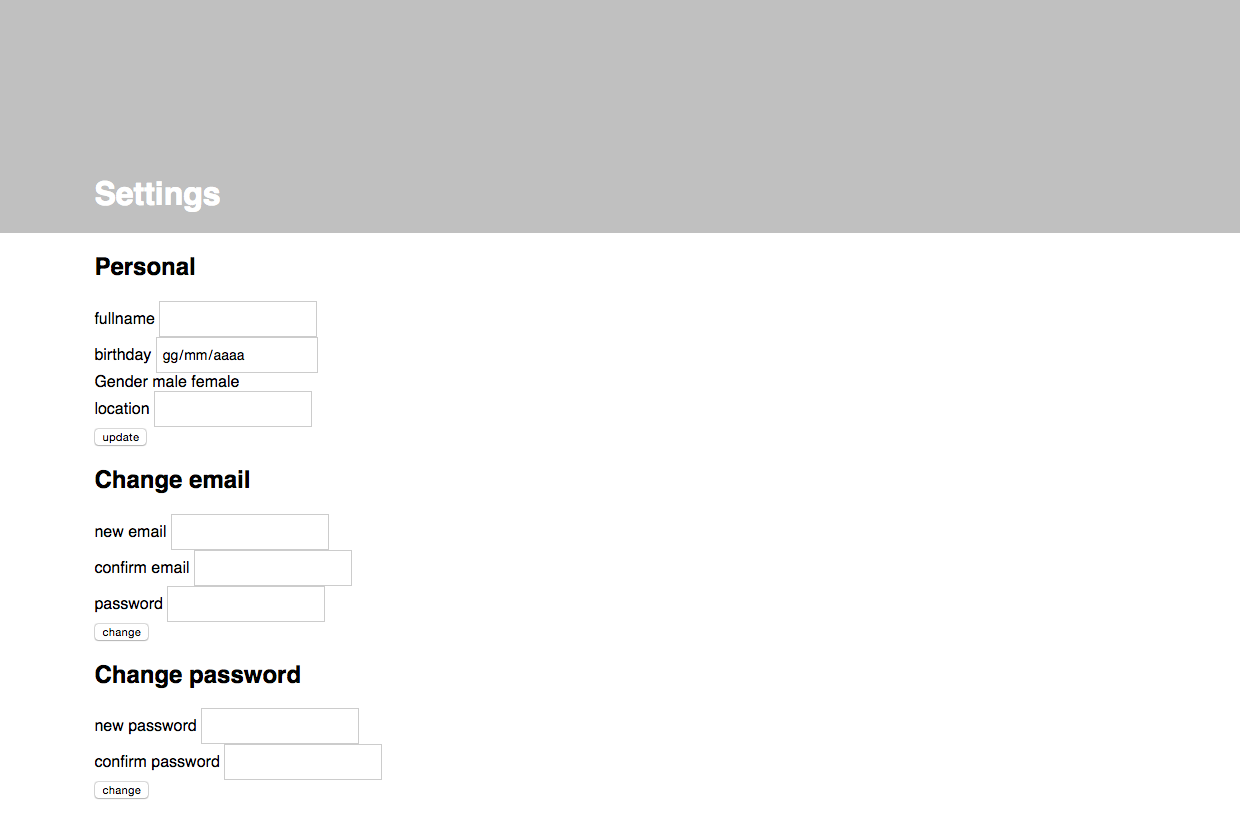
\includegraphics[width=\textwidth]{usr2}
\caption{Settings  Element}
\end {figure}
